\begin{figure}
  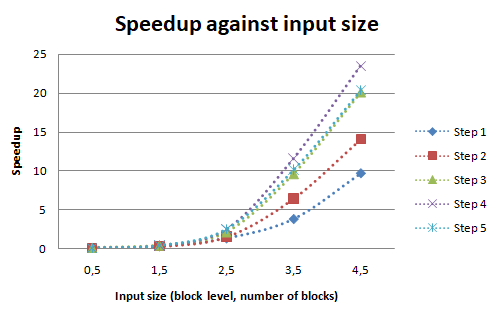
\includegraphics[width=\linewidth]{./images/graph.png}
  \caption{Speedup against input size}
  \label{fig:graph}
\end{figure}
All the above mentioned facts lead to number of stable CUDA implementations for the DENDRO library.
\begin{enumerate}
\item Sending all data blocks to GPU, process them and taking the output as whole
\item Restructuring the format of the input to get better cache optimization
\item Blockwise processing with eliminated intermediate array reallocations
\item Introducing block-wise asynchronous data transfers
\item HtoD and DtoH memory copy overlapping
\end{enumerate}
Below speedup diagram shows that the performance of different implementations mentioned above against the same input block set for level 4.
\\Step 1 is the most basic stable version which gives a speedup of 10.8 with 95\% confidence. On this point, implementation of block-wise processing gave a significant performance gain although couple of other implementations such as cache level optimization and kernel scheduling optimization were ended up with subtle impact on final objective. After that, the implementation of eliminating intermediate memory re-allocation was the major success that led to number of improvements as well. Since memory allocations and deallocation in CUDA are expensive as well as works synchronously, by eliminating a set of those calls returned a very significant performance again. And also it made the whole implementation free from synchronous CUDA API calls. Therefore it allowed to use streams for the system which led to back and forth asynchronous memory transferring. That was the next implementation which increased the speedup further. Final implementation allowed to overlap host to device and device to host memory transfers. In order to do that, output array needs to be on pinned memory on host. Since it needs some amount of time to allocate pinned memory, minor speedup drop can be identified in the last implementation.
\\Another reason to this speedup drop is, this process does not take advantage of HtoD and DtoH memory overlapping since the process is dominated by the computational time. Which means both back and forth memory transfer time is smaller than the computation time of associate block. Refer to Figure \ref{fig:graph} speedup diagram to get further comparison of different implementation against different input sizes.
